\documentclass
  [
    openany,
    math-font    = STIX Two Math,
    main-font    = { {Libertinus Serif} },
    sans-font    = { {Libertinus Sans} },
    mono-font    = { {Libertinus Mono} },
    CJKmain-font =
      { {Zhuque Fangsong (technical preview)} [AutoFakeBold, AutoFakeSlant] },
    CJKsans-font = { {LXGW WenKai} [BoldFont = *-Medium, AutoFakeSlant] },
    CJKmono-font = { {LXGW WenKai Mono} [BoldFont = *-Medium, AutoFakeSlant] },
    % hideanswer   = true,
  ] {whatsnote}

\usepackage{qrcode,magicwatermark,pgfpages}
\MagicWatermark
  {
    setup =
      {
        style = {opacity = .15}, pages = {odd},
        % style = {opacity = .15}, pages = {*},
        content = {\includegraphics[width = .6\linewidth]{WY Logo}},
      },
    setup =
      {
        style = {opacity = .15}, pages = {even},
        content = {\includegraphics[width = .6\linewidth]{7stars_logo}},
      }
  }
% \pgfpagesuselayout{2 on 1}[a3paper, landscape]

\begin{document}

\fancyhead[OL]
  {
    \color{DarkGreen} \href{http://weixin.qq.com/r/DBIABcHEqgnWKIVmb0eI}
      {\faIcon{weixin}~微信公众号：未央学社}
  }
\pagestyle{fancy}

\fancyhead[ER]
  {
    \color{MidnightBlue}\href{https://qm.qq.com/q/j5cuCU4ucw}
      {\faIcon{qq}~未央物理营：782790567}
  }

\chapter*{\sffamily 2024年\textsf{HDU}「大学物理2」期中模拟}

\vspace{-.4\baselineskip}\setcounter{page}{1}
\begin{minipage}{.66\textwidth}
  \centering
  \includegraphics[width = .96\linewidth]{border}
  % \begin{tasks}
  %   [ label-width = 5\ccwd, item-indent = 2cm,
  %     after-item-skip = 0pt ](2)
  %   \task[\textbf{开课学院}：] 理学院
  %   \task[\textbf{解析提供}：] \textsf{Skyrmion}
  %   \task[\textbf{课程编码}：] A0715012
  %   \task[\textbf{\textsf\TeX~排版}：] \textsf{Skyrmion}
  % \end{tasks}
\end{minipage}
\hfill
\begin{minipage}{.15\textwidth}
  \centering
  \begin{tikzpicture}
    \node [ inner sep = 0 ] at (0,0) {
      \qrcode[ height = 4em, version = 4 ]{http://weixin.qq.com/r/sRJiemTEGjllrSAZ90ej}};
    \fill [ white ] (-14em/33,14em/33) rectangle (14em/33,-14em/33);
    \fill [ DarkGreen!60, rounded corners = 4em/33 ]
      (-12em/33,12em/33) rectangle (12em/33,-12em/33);
    \node [ inner sep = 0, white, font = \scriptsize ]
      (weixin) at (0,0) {\faIcon{weixin}};
    \node
      [ inner sep = .5ex, align = center, right,
        xshift = 2em, font = \scriptsize ] at (weixin.east) {未\\央\\学\\社};
  \end{tikzpicture}
\end{minipage}
\begin{minipage}{.15\textwidth}
  \centering
  \begin{tikzpicture}
    \node [ inner sep = 0 ] at (0,0) {
      \qrcode [ height = 4em, version = 4 ]{https://qm.qq.com/q/PH7CsQWvm2}};
    \fill [ white ] (-14em/33,14em/33) rectangle (14em/33,-14em/33);
    \fill [ MidnightBlue!60, rounded corners = 4em/33 ]
      (-12em/33,12em/33) rectangle (12em/33,-12em/33);
    \node [ inner sep = 0, white, font = \scriptsize ]
      (qq) at (0,0) {\faIcon{qq}};
    \node
      [ inner sep = .5ex, align = center, left,
        xshift = -2em, font = \scriptsize ] at (qq.west) {物\\理\\营};
  \end{tikzpicture}
\end{minipage}

\section{选择题（每题3分，共27分）}

\begin{textfig}
  \begin{problem}
    图(a)、(b)、(c)为三个不同的简谐振动系统，组成各系统的各弹簧的原长、劲度系数均相同.
    三个系统的固有角频率平方之比为多少？当图(b)中的物块运动到距平衡点的振幅一半的位置时，
    弹簧的弹性势能与物块的动能之比为多少？
    \begin{tasks}(2)
      \task $1:1:2,~ 1:4$
      \task $2:2:1,~ 1:3$
      \task $2:2:1,~ 1:4$
      \task[\true] $1:1:2,~ 1:3$
    \end{tasks}
  \end{problem}
  \textfigsplit\centering
  \begin{tikzpicture}
    \foreach \a in {0,2,4}
      {
        \draw [ xshift = \a cm ] (-.75,0) -- (.75,0);
        \fill [ pattern = north east lines, xshift = \a cm ]
          (-.75, .2) rectangle (.75,0);
      }
    \node [ draw, rectangle, minimum width = .8cm, minimum height = .4cm ]
      (a) at (0,-2.2) {$m/2$};
    \draw [ decorate, decoration = { coil, segment length = 4pt } ]
      (0,0) -- (a.north)
      node [ near start, right ] {$k$} node [ near end, right ] {$k$};
    \node [ draw, rectangle, minimum width = .8cm, minimum height = .4cm ]
      (b) at (2,-1.2) {$m$};
    \draw [ decorate, decoration = { coil, segment length = 4pt } ]
      (2,0) -- node [ right ] {$k$} (b.north);
    \node [ draw, rectangle, minimum width = .8cm, minimum height = .4cm ]
      (c) at (4,-1.2) {$m$};
    \draw [ decorate, decoration = { coil, segment length = 4pt } ]
      (3.8,0) -- node [ left ] {$k$} ([xshift = -.2cm]c.north);
    \draw [ decorate, decoration = { coil, segment length = 4pt } ]
      (4.2,0) -- node [ right ] {$k$} ([xshift = .2cm]c.north);
    \node [ below ] at (0,-2.5) {(a)} node [ below ] at (2,-2.5) {(b)}
     node [ below ] at (4,-2.5) {(c)};
  \end{tikzpicture}
\end{textfig}
\scratch
\begin{solution}
  三个系统的有效劲度系数分别为 $k_1 = k/2,~ k_2 = k,~ k_3 = 2k$.
  由 $\omega^2 = k/m$ 得固有角频率平方之比为
  $\omega_a^2:\omega_b^2:\omega_c^2 = 1:1:2$.
  当图(b)中的物块运动到距平衡点的振幅一半的位置时，弹簧的弹性势能与物块的动能之比为
  $  E_k/E_p = (E - E_p)/E_p
   = \frac12 k(A/2)^2 \big/ \ab[\frac12 kA^2 - \frac12 k(A/2)^2] = 1/3 $.
  所以本题选择D项.
\end{solution}

\begin{textfig}
  \begin{problem}
    如图所示，用波长 $\lambda = \qty{600}\nm$ 的单色光做杨氏双缝实验，
    在 $P$ 处产生第5级明纹极大，现分别将折射率 $n_1 = 1.75$ 和 $n_2 = 1.25$
    的等厚薄透明玻璃片分别盖在缝 $S_1$ 和 $S_2$ 上，
    此时 $P$ 处变成第一级明纹极大的位置，则玻璃片厚度为
    \begin{tasks}(4)
      \task $\qty{4.8}\um$
      \task $\qty{6.0}\um$
      \task $\qty{7.2}\um$
      \task $\qty{8.4}\um$
    \end{tasks}
  \end{problem}
  \textfigsplit\centering
  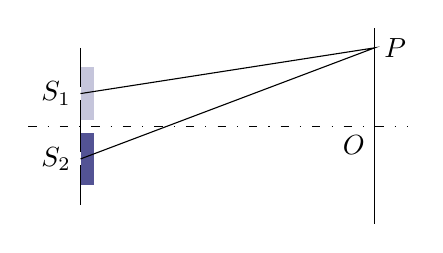
\begin{tikzpicture}[ scale = .83]
    \draw (0,1.2) -- (0,.6);
    \draw (0,.4) -- (0,-.4);
    \draw (0,-.6) -- (0,-1.2);
    \draw [ loosely dash dot ] (-.8,0) -- (5,0);
    \draw (4.5,1.5) -- (4.5,-1.5);
    \fill [ MidnightBlue, opacity = .25 ] (0,.9) rectangle (.2,.1);
    \fill [ MidnightBlue, opacity = .75 ] (0,-.9) rectangle (.2,-.1);
    \draw (0,0.5) -- (4.5,1.2) -- (0,-0.5);
    \node [ left ] at (0,0.5) {$S_1$}
     node [ left ] at (0,-0.5) {$S_2$};
    \node [ right ] at (4.5,1.2) {$P$};
    \node [ below left] at (4.5,0) {$O$};
  \end{tikzpicture}
\end{textfig}
\scratch
\begin{solution}
  遮住前后光程差分别为
  \[
    \begin{cases}
      \delta_1 = 5\lambda = r_2 - r_1\\
      \delta_2 = \lambda = [r_2 + (n_2 - 1)e] - [r_1 + (n_1 - 1)e]
    \end{cases}
  \]
  联立得 $5\lambda - \lambda = \qty{2400}\nm = (n_1 - n_2)e$，
  得玻璃片厚度 $e = \qty{4.8e-4}\cm$. 所以本题选择A项.
\end{solution}

\begin{problem}
  一辆从左向右高速行驶的警车发出频率为 $f_s = \qty{1400}\Hz$ 的警铃，
  警车速度大小为 $\qty{70}{\m/\s}$. 一观察者从右向左移动，速度大小为 $\qty{10}{\m/\s}$.
  假设空气中没有风，空气中的声速 $u = \qty{340}{\m/\s}$.
  观察者与警车相遇前后听到警铃的频率分别为
  \begin{tasks}(4)
    \task $\qty{1711.1}\Hz,~ \qty{1195.1}\Hz$
    \task $\qty{1126.8}\Hz,~ \qty{1814.8}\Hz$
    \task[\true] $\qty{1814.8}\Hz,~ \qty{1126.8}\Hz$
    \task $\qty{1196.1}\Hz,~ \qty{1711.1}\Hz$
  \end{tasks}
\end{problem}
\scratch
\begin{solution}
  已知多普勒效应观察者 (Observer) 和发射源 (Source) 的频率关系为
  \[\nu = \frac{u\pm v_o}{u\mp v_s}\nu_0\]
  $v_o$ 为观察者速度，接近为 $+$，远离为 $-$；
  $v_s$ 为发射源速度，接近为 $-$，远离为 $+$. 观察者所听频率分别为
  \[
    f_1 = \frac{340 + 10}{340 - 70} \times \qty{1400}\Hz
        \approx \qty{1814.8}\Hz,~
    f_2 = \frac{340 - 10}{340 + 70} \times \qty{1400}\Hz
        \approx \qty{1126.8}\Hz
  \]
  所以本题选择C项.
\end{solution}

\begin{textfig}
  \begin{problem}[波的能量]
    图示为一平面简谐机械波在 $t$ 时刻的波形曲线. 若此时 $A$ 点处媒质质元的振动动能在增大，则
    \begin{tasks}(2)
      \task $A$ 点处质元的弹性势能减小
      \task[\true] 波沿 $x$ 轴负方向传播
      \task $B$ 点处质元的振动动能增大
      \task 各点能量密度都不含时
    \end{tasks}
  \end{problem}
  \textfigsplit\centering
  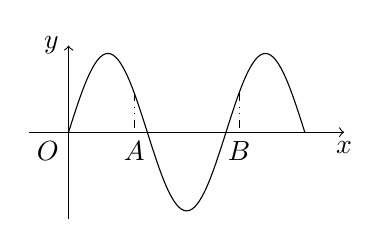
\begin{tikzpicture}
    \draw [ -> ] (-.5,0) -- (3.5,0) node [ below ] {$x$};
    \draw [ -> ] (0,-1.1) -- (0,1.1) node [ left ] {$y$};
    \draw (0,0) sin (.5,1) cos (1,0) sin (1.5,-1)
      cos (2,0) sin (2.5,1) cos (3,0);
    \node [ below left ] at (0,0) {$O$};
    \draw [ dash dot dot] (5/6,.5) -- (5/6,0) node [ below ] {$A$};
    \draw [ dash dot dot ] (13/6,.5) -- (13/6,0) node [ below ] {$B$};
  \end{tikzpicture}  
\end{textfig}
\begin{solution}\leavevmode
  \begin{itemize}
    \item $A$ 点的振动动能在增大，所以 $A$ 点在靠近平衡位置，
    波沿 $x$ 轴负方向传播，B选项正确.
    \item 波沿 $x$ 轴负方向传播，由图可知 $B$ 点在远离平衡位置，其振动动能在减小，
    C选项错误.
    \item 根据机械波的特性：动能和势能同时增大或减小，能量密度随时间变化，AD选项错误.
  \end{itemize}
\end{solution}

\begin{problem}[迈克尔逊干涉仪]
  在迈克尔逊干涉仪的一条光路中，放入一折射率为 $n$，厚度为 $d$ 的透明薄片.
  放入后，这条光路的光程改变了
  \begin{tasks}(5)
    \task[\true] $2(n - 1)d$
    \task $2nd$
    \task $2(n - 1)d + \frac\lambda2$
    \task $nd$
    \task $(n - 1)d$
  \end{tasks}
\end{problem}
\scratch
\begin{solution}
  迈克尔逊干涉仪光路上的某点光碰到反射镜后会再次经过此处，故原来的光程为 $2d$；
  现在加入了透明薄片，使得这里的光程为 $2nd$，故光程差为 $2(n - 1)d$. 所以本题选择A项.
\end{solution}

\begin{textfig}
  \begin{problem}
    在双缝干涉实验中，用白光照射双缝隙，屏幕 $E$ 上的 $P$ 点明条纹外侧呈什么颜色？
    如果用纯绿色滤光片和纯蓝色滤光片分别盖住两缝，能否产生干涉条纹？
    若将缝 $S_2$ 盖住，并在 $S_1S_2$ 连线的垂直平分面处放一高折射率反射面$M$，如图所示.
    则此时P点是明纹还是暗纹？
    \begin{tasks}(2)
      \task 红色，能，明纹
      \task 蓝色，能，暗纹
      \task 蓝色，不能，明纹
      \task[\true] 红色，不能，暗纹
    \end{tasks}        
  \end{problem}
  \textfigsplit\centering  
  \begin{tikzpicture}
    [ decoration = { markings, mark = at position .2 with \arrow{stealth'} } ]
    \draw [ very thick ] (0,1.5) -- (0,-1.5);
    \draw [ postaction = decorate ] (-1,0) -- (0,.5) -- (2,.8);
    \draw (0,.5) -- (.8,0);
    \draw [ postaction = decorate ] (-1,0) -- (0,-.5) -- (2,.8);
    \draw [ very thick ] (0,0) -- (1.8,0);
    \draw [ very thick ] (2,1.8) -- (2,-1.8);
    \fill [ pattern = north west lines ] (0,0) rectangle (1.8,-.2);
    \fill [ pattern = north east lines ] (2,1.8) rectangle (2.2,-1.8);
    \node [ left ] at (-1,0) {$S$} node [ above left ] at (0,.5) {$S_1$}
     node [ below left ] at (0,-0.5) {$S_2$};
    \node [ below ] at (0.8,-0.2) {$M$} node [ right ] at (2.2,0.8) {$P$}
     node [ below ] at (2.1,-1.8) {$E$};
    \node at (-1,0) {\ensuremath\times};
  \end{tikzpicture}
\end{textfig}
\begin{solution}\leavevmode
  由于波长越大，明纹张角越大，所以外侧呈红色. 根据干涉条件「频率相等」，此时不能产生干涉条纹.
  添加反射面后，虽然光路长度不变，但使反射导致光路 $S_1MP$ 存在半波损失，
  两条光路的相位差变化 $\pi$，所以 $P$ 点由明纹变为暗纹. 所以本题选择A项.
\end{solution}

\begin{textfig}
  \begin{problem}
    如图所示，两个直径有微小差别的彼此平行的滚柱之间的距离为 $L$，夹在两块平板透光晶体的中间，
    形成空气劈尖. 当单色光垂直入射时，产生等厚干涉条纹，如果两滚柱之间的距离 $L$ 变小，
    或同时等比缩小两滚柱的半径，两种情况下则在 $L$ 范围内干涉条纹的间距和级数分别会怎样？
      \begin{tasks}(2)
        \task 变大，减小；不变，变小
        \task[\true] 变小，不变；不变，变小
        \task 变小，不变；变小，变大
        \task 变小，增加；变大，变大
      \end{tasks}
    \end{problem}
    \textfigsplit\centering
    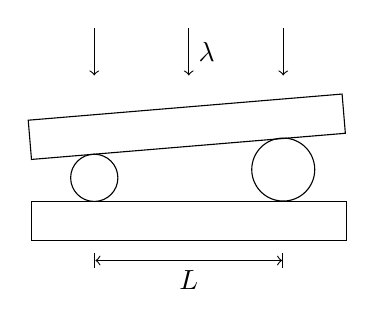
\begin{tikzpicture}
      \draw (-2,0) rectangle + (4,0.5);
      \draw (-1.2,0.8) circle (0.3);
      \draw (1.2,0.905) circle (0.4);
      \draw [ rotate around = {atan(1/12):(-1.2,1.1)} ]
        (-2,1.1) rectangle + (4,0.5);
      \draw [ |<->| ] (-1.2,-.25) -- node [ below ] {$L$} (1.2,-.25);
      \foreach \a in {-1.2,0,1.2}
        \draw [ ->, xshift = \a cm ] (0,2.7) -- (0,2.1);
      \node [ right ] at (0,2.4) {$\lambda$};
    \end{tikzpicture}
\end{textfig}
\begin{solution}
  两滚筒间距变小相当于劈尖的顶角变大，
  根据条纹间距公式 $\Delta x = \lambda/2\theta$ 可知条纹间隔变小；
  对于某条纹路，其光程差是确定的，所以数目不变.
  缩小过程中空气劈形膜的顶角不变，所以条纹间隔不变，但每处的光程差减小，
  所以对应的条纹级数减小. 所以本题选择B项.
\end{solution}

\begin{problem}
  在单缝夫琅和费衍射实验中，波长为 $\lambda$ 的单色光垂直入射在宽度为
  $a = 6\lambda$ 的单缝上，对应于衍射角为 $\qty{30}\degree$ 的方向，
  单缝处波阵面可分成的半波带数目为
  \begin{tasks}(4)
    \task $2$个
    \task $4$个
    \task[\true] $6$个
    \task $8$个
  \end{tasks}
\end{problem}
\begin{solution}
  由衍射公式 $a\sin\theta = k\lambda$ 得 $k = 3$，可分成的半波带数目为 $2k = 6$.
  所以本题选择C项.
\end{solution}

\begin{textfig}
  \begin{problem}
    在如图所示的单缝弗琅禾费衍射装置中，将单缝宽度 $a$ 稍稍变宽，
    同时使单缝沿 $y$ 轴正方向做微小平移（透镜屏幕位置不动），则屏幕 $C$ 上的中央衍射条纹将
    \begin{tasks}(2)
      \task 变窄，同时向上移
      \task 变窄，同时向下移
      \task[\true] 变窄，不移动
      \task 变宽，同时向上移
    \end{tasks}
  \end{problem}
  \textfigsplit\centering
  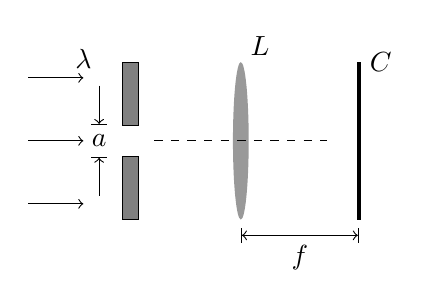
\begin{tikzpicture}
    \foreach \y in {0.8,0,-0.8}
      \draw [ ->, yshift = \y cm ] (-1.2,0) -- (-.5,0);
    \node [ above ] at (-0.5,0.8) {$\lambda$};
    \filldraw [ fill = gray ] (0,1) rectangle (.2,.2);
    \filldraw [ fill = gray ] (0,-1) rectangle (.2,-.2);
    \draw [ ->| ] (-.3,.7) -- (-.3,.2);
    \draw [ ->| ] (-.3,-.7) -- (-.3,-.2);
    \node at (-.3,0) {$a$};
    \fill [ opacity = .4 ] (1.5,0) ellipse (.1 and 1);
    \node [ right ] at (1.5,1.2) {$L$};
    \draw [ |<->| ] (1.5,-1.2) -- node [ below ] {$f$} (3,-1.2);
    \draw [ dashed ] (.4,0) -- (2.6,0);
    \draw [ very thick ] (3,1) node [ right ] {$C$} -- (3,-1);
  \end{tikzpicture}
\end{textfig}
\begin{solution}
  光线方向不变，所以中央明纹位置不变；
  根据中央明纹宽度 $\Delta x_0 = 2\lambda f/a$ 可知单缝宽度增大，中央明纹宽度将变窄.
  所以本题选择C项.
\end{solution}

\section{填空题（共27分）}

\begin{problem}[本题3分]
  在 $t = 0$ 时，振幅为 $A$，周期为 $T$ 的单摆分别处于做左下方图示的三种状态.
  若选单摆的平衡位置为坐标原点，坐标指向正右方，
  则单摆做小角度摆动的振动表达式（用余弦函数表示）分别为
  \begin{enumerate*}[ label = (\alph*) ]
    \item \result{$x = A\cos(2\pi t/T - \pi/2)$}
    \item \result{$x = A\cos(2\pi t/T + \pi/2)$}
    \item \result{$x = A\cos(2\pi t/T + \pi)$}.
  \end{enumerate*}
\end{problem}
\begin{solution}
  三种情况对应的相位分别为 $x = 0,~ v > 0,~ \varphi = -\frac\pi2$；
  $x = 0,~ v < 0,~ \varphi = \frac\pi2$；$x = -A,~ v = 0,~ \pi$.
  所以振动表达式分别为
  $A\cos(2\pi t/T - \pi/2),~ A\cos(2\pi t/T + \pi/2),~ A\cos(2\pi t/T + \pi)$.
\end{solution}

\begin{textfig}[ lefthand ratio = .5 ]
  \centering
  \begin{tikzpicture}
    \foreach \a in {0,2,4}
      {
        \draw [ xshift = \a cm ] (-.75,0) -- (.75,0);
        \fill [ pattern = north east lines, xshift = \a cm]
          (-.75,0) rectangle (.75,.2);
      }
    \draw (0,0) -- (0,-2);
    \draw [ -> ] (0,-2) --++ (.6,0) node [ above ] {$v_0$};
    \shade [ ball color = MidnightBlue ] (0,-2) circle (0.1);
    \node [ below ] at (0,-2.4) {(a)};

    \draw (2,0) -- (2,-2);
    \draw [ -> ] (2,-2) --++ (-.6,0) node [ above ] {$v_0$};
    \shade [ ball color = MidnightBlue ] (2,-2) circle (0.1);
    \node [ below ] at (2,-2.4) {(b)};
  
    \draw [ dashed ] (4,0) -- (4,-2);
    \draw (4,0) -- (3,-2) node [ below ] {$v_0 = 0$};
    \shade [ ball color = MidnightBlue ] (3,-2) circle (0.1);
    \node [ below ] at (4,-2.4) {(c)};
  \end{tikzpicture}
  \textfigsplit\centering
  \begin{tikzpicture}
    [ decoration = 
      { markings,
        mark = between positions 0.05 and 1 step 6mm with
          {\draw [ -, darkgray ] (0,-0.1) -- (0,0.1);}
      }
    ]
      \draw [ ->, postaction = decorate ] (-.2,0) -- (4.2,0)
       node [ above ] {$x/\unit\m$};
      \draw [ -> ] (0,-1.2) -- (0,1.5) node [ left ] {$y/\unit\m$};
      \node [ below left ] at (0,0) {$O$};
      \draw (0,0) sin (0.6,-1) cos (1.2,0) sin (1.8,1)
        cos (2.4,0) sin (3,-1) cos (3.6,0);
      \draw [ very thick, -> ] (2,1.2) --
       node [ above ] {$u = \qty{0.08}{\m/\s}$} (3.2,1.2);
      \node [ below ] at (0.6,0) {$0.1$} node [ below ] at (1.8,0) {$0.3$}
       node [ below ] at (3,0) {$0.5$};
      \draw [ dashed ] (0,1) node [ left ] {$0.04$} -- (1.8,1);
  \end{tikzpicture}
\end{textfig}

\begin{problem}[本题3分]
  右上方图所示为一平面简谐波在\emph{ $t = \qty2\s$ }时的波形图，
  则 $O$ 点的振动方程为 $y_o = $\result{$0.04\cos(0.4\pi t - 1.3\pi)$}.
\end{problem}
\begin{solution}
  由图可知 $A = \qty{0.04}\m$，$\lambda = \qty{0.4}\m$，
  $\omega = 2\pi u/\lambda = 0.4\pi$.
  此时 $O$ 点处质点速度 $v > 0$，此时其相位为 $\varphi_0 = -\pi/2$，
  $t = 0$ 时其的相位为 $\varphi = \varphi_0 - \omega \times 2 = -1.3\pi$.
  综上所述，$O$ 点的振动方程 $y_o = 0.04\cos(0.4\pi t - 1.3\pi)$.
\end{solution}

\begin{problem}[本题2分]
  光强均为 $I_0$ 的两束相干光干涉时，在相遇区域内可能出现的最大光强是\result{$4I_0$}，
  可能出现的最小光强是\result{$0$}.
\end{problem}
\scratch
\begin{solution}
  两种情况分别为「干涉相长」与「干涉相消」，由 $I = I_1 + I_2 \pm 2\sqrt{I_1I_2}$
  得光强分别为 $4I_0$ 与 $0$.
\end{solution}

\begin{problem}[本题2分]
  若在迈克尔逊干涉仪的可动反射镜 $M$ 移动 $\qty{0.644}\mm$ 过程中，
  观察到干涉条纹移动了 $2048$ 条，则所用光波的波长为\result{$\qty{628.9}\nm$}.
\end{problem}
\begin{solution}
  移动带来的光程差满足 $\delta = 2d = N\lambda$，
  由此得 $\lambda = 2d/N = \qty{628.9}\nm$.
\end{solution}

\begin{problem}[本题5分]
  一平面简谐波沿 $Ox$ 轴正方向传播，波长为 $\lambda$，
  若位于 $x = -L_1$ 的 $P_1$ 处质点的振动方程为 $y_1 = A\cos(2\pi\nu t + \phi)$，
  则位于 $x = L_2$ 的 $P_2$ 处质点的振动方程为
  \result{$y_2 = A\cos[2\pi(\nu t - (L_2 + L_1)/\lambda) + \phi]$}；
  与 $P_1$ 处质点振动状态相同的那些点的位置为
  \result{$x = -L_1 + k\lambda,~ k = 0,~ \pm 1,~ \pm 2,~ \cdots$}.
\end{problem}
\scratch[3ex]
\begin{solution}
  将 $P_1$ 点的振动方程中加入传播项得波函数
  \[
    y = A\cos\ab\{2\pi\nu t - \frac{2\pi[x - (-L_1)]}{\lambda} + \phi\}
      = A\cos\ab[2\pi\nu t - \frac{2\pi(x + L_1)}{\lambda} + \phi]
  \]
  令 $x = L_2$，得 $P_2$ 点的振动方程
  $y_2 = A\cos\ab[2\pi\nu t - \frac{2\pi(L_2 + L_1)}{\lambda} + \phi]$
  与点 $P_1$ 处质点振动状态相同的点与 $P_1$ 点的距离应为波长的整数倍，
  即 $x = -L_1 + k\lambda,~ k = 0,~ \pm 1,~ \pm 2,~ \cdots$.
\end{solution}

\begin{problem}[本题3分]
  两个同方向简谐振动的振动方程分别为
  $ x_1 = \num{5e-2}\cos\ab(10t + \frac34\pi),~
    x_2 = \num{6e-2}\cos\ab(10t + \frac14\pi)
  $，则合振动方程为\result{$x = \num{7.81e-2}\cos(10t + 0.47\pi)$}.
\end{problem}
\scratch[1ex]
\begin{solution}\leavevmode
  \begin{itemize}
    \item 合振动振幅为
    $ A = \sqrt{A_1^2 + A_2^2 + 2A_1A_2\cos(\varphi_1 - \varphi_2)}
        = \qty{7.8e-2}\m$.
    \item 合振动相位
    $\varphi = \arctan[
        (A_1\sin\varphi_1 + A_2\sin\varphi_2)/
        (A_1\cos\varphi_1 + A_2\cos\varphi_2)
      ] = 0.47\pi$.
    \item 两者振动频率相同，所以合振动频率与其相同.
    故合振动方程为 $x = \num{7.8e-2}\cos(10t + 0.47\pi)$.
  \end{itemize}
\end{solution}

\begin{textfig}
  \begin{problem}[本题2分]
    两相干波源 $S_1$ 和 $S_2$ 相距 $\lambda/4$，$S_1$ 的相位比 $S_2$ 超前 $\pi/2$.
    则图中两波引起的简谐振动在 $P$ 点的相位差是\result{$\pi$}.
  \end{problem}
  \textfigsplit\centering
  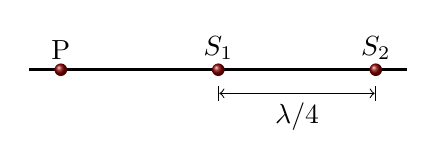
\begin{tikzpicture}
    \draw [ very thick ] (-2.4,0) -- (2.4,0);
    \draw [ |<->| ] (0,-.3) -- node [ below ] {$\lambda/4$} (2,-.3);
    \foreach \a in {-2,0,2}
      \shade [ ball color = DarkRed ] (\a,0) circle (.08);
    \node [ above ] at (-2,0) {P};
    \node [ above ] at (0,0) {$S_1$};
    \node [ above ] at (2,0) {$S_2$};
  \end{tikzpicture}
\end{textfig}
\begin{solution}
  传播带来的相位差为 $2\pi\delta/\lambda = \pi/2$，
  波源 $S_1$ 比 $S_2$ 的相位超前 $\pi/2$，所以 $P$ 点处相位差为 $\pi$.
\end{solution}

\begin{problem}[本题3分]
  一束波长为 $\lambda = \qty{600}\nm$ 的平行单色光垂直入射到折射率为 $n$ 的透明薄膜上，
  \textbf{该膜是放在空气中的}. 要使\textbf{透射光}得到最大限度的\textbf{加强}，
  薄膜最小厚度应为\result{$\lambda/2n$}.
\end{problem}
\scratch
\begin{solution}
  \textbf{当光从光密介质射向光疏介质时，反射光没有半波损失}.
  所以两个表面反射光光程差为 $\delta = 2ne - \lambda/2$. 要使透射光得到最大限度的加强，
  可使反射光满足干涉相消条件 $2ne - \lambda/2 = (2k + 1)\lambda/2$.
  当 $k = 0$ 时，薄膜满足最小厚度 $e_{\min} = \lambda/2n$.
\end{solution}

\begin{problem}[本题4分]
  用波长 $\qty{500}\nm$ 的单色光垂直照射到由两块光学平玻璃构成的空气劈形膜上.
  在观察反射光的干涉现象中，
  距劈形膜棱边 $l = \qty{1.56}\cm$ 的 $A$ 处是从棱边算起的第四条暗纹中心.
  此空气劈形膜的劈尖角 $\theta = $\result{$\qty{4.8e-15}\radian$}；
  若改用 $\qty{600}\nm$ 的单色光垂直照射到此劈尖上仍观察反射光的干涉条纹，
  $A$ 处是\result{明纹}，
  此时从棱边到 $A$ 处的范围共有\result{$3$}条明纹，\result{$3$}条暗纹.
\end{problem}
\scratch[2ex]
\begin{solution}\leavevmode
  \begin{enumerate}
    \item 考虑半波损失，两束光的光程差为 $\delta = 2h_k + \frac\lambda2$，由暗纹条件
      \[
          2h_4 + \frac\lambda2 = \frac{2k - 1}{2}\lambda
        = \frac{2 \times 4 - 1}{2}\lambda
      \]
      利用小角度近似得劈尖角
      $\theta\approx\frac{h_4}{l} = \qty{4.81e-5}\radian,~ h_4 = \qty{750}\nm$.
    \item 此时光程差
    $\delta = 2h_4 + \frac{\lambda'}{2} = \qty{1800}\nm = 3\lambda'$，
    满足明纹条件$\delta = k\lambda$. 所以$A$处是第3条明纹.
    \item 由棱边处的光程差 $\delta = \frac\lambda2$ 可知棱边处为暗纹.
    所以共有 $3$ 条明纹，$3$ 条暗纹.
  \end{enumerate}
\end{solution}

\section{计算题（共46分）}

\begin{problem}[本题5分]
  某质点做简谐振动，周期为 $\qty3\s$，振幅为 $\qty{0.5}\m$，$t = \qty{0.75}\s$ 时刻，
  质点恰好处在 $x = \frac{\sqrt2}{2}A$ 位置并向负方向运动，求
  \begin{enumerate}
    \item 该质点的振动方程.
    \item 此振动以速度 $u = \qty5{\m/\s}$ 沿 $x$ 轴负方向传播时，
    形成的一维简谐波函数（以平衡位置为坐标原点）.
    \item 该波的波长.
  \end{enumerate}
\end{problem}
\scratch[1em]
\begin{solution}\leavevmode
  \begin{enumerate}
    \item 由题意得，质点的角频率 $\omega = 2\pi/T = 2\pi/3$，
    质点的初相 $\varphi = \pi/4$. 故质点的振动方程为
    \[
      y_0 = 0.5\cos\ab[\frac23\pi(t - 0.75) + \frac\pi4]
          = 0.5\cos\ab(\frac23\pi t - \frac\pi4)\]
    \item 在振动方程中加入传播项 $+x/u$ 得波函数
    $ y = A\cos\ab[\omega\ab(t + \frac xu) + \varphi]
        = 0.5\cos\ab[\frac23\pi\ab(t + \frac x5) - \frac\pi4]$.
    \item 波长 $\lambda = uT = \qty{15}\m$.
  \end{enumerate}
\end{solution}

\begin{problem}[本题5分]
  薄钢片上有两条紧靠的平行细缝，
  用波长 $\lambda = \qty{546.1}\nm$ 的平面光波正入射到钢片上. 
  屏幕距双缝的距离为 $D = \qty{2.00}\m$，
  测得中央明纹两侧的第五级明纹间的距离为 $\Delta x = \qty{12.0}\mm$.
  \begin{enumerate}
    \item 求两缝间的距离.
    \item 如果使光波斜入射到钢片上，条纹间距将如何改变？
  \end{enumerate}
\end{problem}
\scratch[4ex]
\begin{solution}\leavevmode
  \begin{enumerate}
    \item 由明纹坐标公式 $x = \frac{k\lambda D}{d}$ 得两侧第五级明纹间隔
    $\Delta x_5 = \frac{10\lambda D}{d}$，
    $d = \frac{10\lambda D}{x} = \qty{0.91}\mm$.
    \item 斜入射只会使所有明纹对应的光程差同时改变 $a\sin\theta$，
    但是相对位置不变，所以条纹间距不变.
  \end{enumerate}
\end{solution}

\begin{problem}[本题7分]
  牛顿环装置透镜凸表面的曲率半径是 $R = \qty{400}\cm$.用某单色平行光垂直入射，
  观察反射光形成的牛顿环，测得第5个明环的半径是 $\qty{0.30}\cm$.
  \begin{enumerate}
    \item 求入射光的波长. 当透镜垂直向上缓慢平移远离平面玻璃时，
    可以观察到环状干涉条纹\result{向中心收缩}.
    \item 若将装置浸泡在折射率 $n = 1.25$ 的溶液中，
    求以透镜中心为圆心在半径为 $\qty1\cm$ 的范围内的明环数目.
    \item 第三级明纹与第七级明纹所对应的空气膜厚度之差为多少？
  \end{enumerate}
\end{problem}
\scratch[4ex]
\begin{solution}\leavevmode
  \begin{enumerate}
    \item 由明环半径公式 $r_k = \sqrt{(2k - 1)\lambda R/2}$
    得入射光的波长 $\lambda = \frac{2r^2}{(2k - 1)R} = \qty{500}\nm$.
    \item 相当于单色光的波长变为 $\lambda' = \frac\lambda n$.
    由明环半径公式，代入 $r = \qty1\cm$
    得 $k = \frac{r^2}{\lambda' R} + \frac12 = 63$.
    \item 由明环半径公式 $r_k = \sqrt{(2k - 1)\lambda R/2}$
    得第三级明纹与第七级明纹所对应的空气膜厚度之差为
    \[
        \Delta d = \sqrt{R^2 - r_3^2} - \sqrt{R^2 - r_7^2}
      = \sqrt{R^2 - \frac52\lambda R} - \sqrt{R^2 - \frac{13}{2}\lambda R}
      \xlongequal{\lambda \ll R} 2\lambda = \qty1\um
    \]
  \end{enumerate}
\end{solution}

\begin{problem}[本题6分]
  一轻弹簧下悬挂 $m_0 = \qty{100}\g$ 砝码时，弹簧伸长 $\qty8\cm$.
  现在这根弹簧下端悬挂 $m = \qty{250}\g$ 的物体构成弹簧振子.
  将物体从平衡位置向下拉动 $\qty4\cm$，并给以向上 $\qty{21}{\cm/\s}$ 的初速度
  （令此时 $t = 0$）. 选 $x$ 轴向下为正方向，求振动方程的数值式.
\end{problem}
\scratch[4ex]
\begin{solution}\leavevmode
  \begin{itemize}
    \item 弹簧的劲度系数、角频率分别为 $k = m_0g/\Delta x_0 = \qty{12.5}{\N/\m},~
    \omega = \sqrt{k/m} = \qty{7.07}\s$.
    \item 由旋转矢量法得系统振幅、初相为
    $A = \sqrt{x_0^2 + (v_0/\omega)^2} = \qty{4.98}\cm,~
    \varphi_0 = \arccos{\frac{x_0}{A}} = 0.20\pi$.
    \item 振动方程为 $y = \num{4.98e-2}\cos(7.07t + 0.20\pi)$.
  \end{itemize}
\end{solution}

\begin{problem}[本题8分]
  设入射波的表达式为 $y_1 = A\cos\ab[2\pi\ab(\frac tT + \frac x\lambda)]$，
  在 $x = 0$ 固定端发生反射，设反射时无能量损失. 求
  \begin{tasks}[ label = \arabic*. ](3)
    \task 反射波的表达式.
    \task 驻波的表达式.
    \task 波腹、波节的位置.
    \task! 任一波节两侧任意两点（两点距离小于 $\lambda/2$）的相位差为\result{$\pi$}.
  \end{tasks}
\end{problem}
\scratch[4ex]
\begin{solution}\leavevmode
  \begin{enumerate}
    \item 到达反射端后，波的传播方向发生变化，同时因半波损失带有 $\pi$ 的相位差.
    所以反射波的表达式为
    \[y_2 = A\cos\ab[2\pi\ab(\frac tT - \frac x\lambda) + \pi]\]
    \item 驻波表达式
    $ y = y_1 + y_2
        = 2A\cos\ab(\frac{2\pi t}{T} + \frac\pi2)
            \cos\ab(\frac{2\pi x}{\lambda} - \frac\pi2)$.
    \item 
    波腹的位置 $\cos\ab(\frac{2\pi x}{\lambda} - \frac\pi2) = \pm 1,~
    x = \frac{2k+1}{4}\lambda,~ k = 0,~ 1,~ 2,~ \ldots$.

    波节的位置 $\cos\ab(\frac{2\pi x}{\lambda} - \frac\pi2) = 0,~
    x = \frac k2\lambda,~ k = 0,~ 1,~ 2,~ \ldots$.
    \item 波节两侧两点处质元的振动方向相反，相位差为 $\pi$.
  \end{enumerate}
\end{solution}

\begin{problem}[本题8分]
  波长为 $\qty{760}\nm$ 的平行光垂直地入射于一宽为 $\qty{0.5}\mm$ 的狭缝，
  若在缝的后面有一焦距为 $\qty2\m$ 的薄透镜，使光线会聚于一屏幕上，试求
\begin{enumerate}
  \item 中央明纹和旁边第一个亮纹的宽度.
  \item 第一级明纹的位置，两侧第二级暗纹之间的距离（$\qty1\nm = \qty{e-9}\m$）.
  \item 若换用白光照射，其中某一光波的第四级明纹和红光（$\lambda = \qty{600}\nm$）
  的第三级明纹相重合，求这一光波的波长.
\end{enumerate}
\end{problem}
\scratch[4ex]
\begin{solution}\leavevmode
  \begin{enumerate}
    \item 中央明条纹宽度 $\Delta x_0 = \frac{2\lambda f}{a} = \qty{6.08}\mm$.
    \item 第一级明纹位置 $a\sin\varphi = \pm(2k + 1)\frac\lambda2$，
    $x_1 = f_1\sin\varphi = \qty{\pm 4.56}\mm$.
        
    第二级暗纹位置
    $ a\sin\varphi = \pm k\lambda,~
      \Delta x_2 = 2 \cdot \frac{2\lambda}{a}f = \qty{12.16}\mm$.
    \item 明纹位置 $a\sin\varphi = \pm\frac{2k + 1}{2}\lambda$，
    由重合条件
    $\frac{2 \times 3 + 1}{2}\lambda = \frac{2 \times 4 + 1}{2}\lambda'$
    得光波波长 $\lambda' = \frac79\lambda = \qty{446.7}\nm$.
  \end{enumerate}
\end{solution}

\end{document}